%TEX root = ./overwiew.tex

\documentclass[varwidth]{standalone}
\usepackage{tikz}
\usetikzlibrary{positioning}

\begin{document}
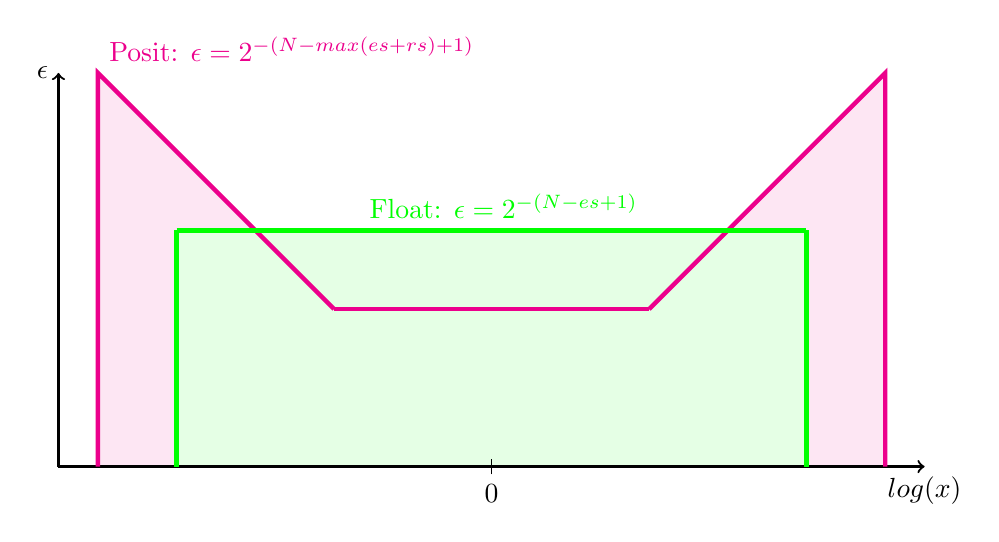
\begin{tikzpicture}[domain=-1:15]
	% Posit
-	\fill [magenta!10, fill opacity=1] (-0.5,0) -- (-0.5,5) -- (2.5,2) -- (6.5,2) -- (9.5,5) -- (9.5, 0) -- cycle;
	% Float
	\fill [green!10, domain=0:8,fill opacity=1] (0.5,0) -- (0.5,3) -- (8.5,3) -- (8.5,0);

	\draw [thick] [->] (-1,0)--(10,0) node[right, below] {$log(x)$};
	\draw [thick] [->] (-1,0)--(-1,5) node[above, left] {$\epsilon$};
	\draw [] (4.5,-0.1) -- (4.5,0.1) node[below=0.2cm] {0};

	% Posit
	\draw [magenta, ultra thick] (-0.5,0) -- (-0.5,5) node[above right] {Posit: $\epsilon=2^{-(N-max(es+rs)+1)}$} -- (2.5,2);
	\draw [domain=2.5:6.5, variable=\x, magenta, ultra thick] plot ({\x}, 2);
	\draw [magenta, ultra thick] (6.5,2) -- (9.5,5) -- (9.5, 0);

	% Float
	\draw [green, ultra thick] (0.5,0) -- (0.5,3);
	\draw [domain=0.5:8.5, variable=\x, green, ultra thick] plot({\x}, 3) node [above left=0cm and 2cm] {Float: $\epsilon = 2^{-(N-es+1)}$};
	\draw [green, ultra thick] (8.5,3) -- (8.5,0);
\end{tikzpicture}
\end{document}

